\section{Method}\label{sec:method}

In this section, we first formulate our problem mathematically and elaborate our approach detailedly in \cref{sec:method_1}.
%
Then we specify how \method can be used in three tasks where the settings are not exactly the same, \textit{i.e.}, fully-supervised, semi-supervised, domain adaptive settings, in \cref{sec:method_2}, \cref{sec:method_3}, \cref{sec:method_4}, respectively.


\subsection{Elaboration of \method}\label{sec:method_1}
Long-tailed label distribution is detrimental to the training of deep learning models.
%
As \cref{fig:stats}a illustrated the total numbers of instances from tail categories are extremely much fewer when compared to head categories.
%
As a result, they are squeezed into a very small area in the feature space,
%
which means \textit{the decision boundaries of these tailed categories can be severely biased}.
%
Thus, at the inference stage, many similar data outside the distribution of the training tail category instances will be misclassified due to this squeeze.
%
Next, we will elaborate on our approach.


Given a long-tailed training dataset with $N$ labeled images of $C$ categories: $D=\left\{(x_{image}^{i}, y_{image}^{i})\right\}_{i=1}^{N}$, where $y_{image}^{i}\in \left\{0, 1, ..., C-1\right\}$,  
%
our goal is to train a semantic segmentation model $f_{model}$ with more balanced representations.
%
To achieve this, we need to take a more fine-grained perspective.
%
For segmentation tasks, the corresponding task-related instances are pixels, instead of images.
%
Thus we can view the task as a multi-label classification task at the pixel level.
%

%
During the training stage, assuming there is an input data batch $X_{batch}$ with a shape of $\left\{B, 3, H, W\right\}$ and its corresponding label $Y_{batch}$, where $B$ is the batch size and $H, W$ denotes the size of the images, we can input it into the model $f$ to get an output vector $\tilde{Z}_{batch}$.
%
The shape of $\tilde{Z}_{batch}$ will be $\left\{B, C, H, W\right\}$ (we assume that $H, W$ remain the same here for simplicity because $\tilde{Z}_{batch}$ can be upsampled to this size), where $C$ is the number of categories.
%

From the view of instances (\textit{i.e.}, pixels in segmentation task), we can reshape the output $\tilde{Z}_{batch}$ from $\left\{B, C, H, W\right\}$ into $\left\{B\times H \times W, C\right\}$.
%
So for this batch, we have $B\times H \times W$ pixels and corresponding $C$-dimensional prediction for each of them.
%
Taking pixel $i$ as an example, its output $\tilde{Z}_{batch}^{i} = \left[z_{0}^{i}, z_{1}^{i}, \cdots, z_{C-1}^{i}\right]$.
%
In order to calculate the cross entropy loss during training, we need to convert it into probabilities by the \texttt{softmax} formula \cref{eq:softmax}.
\begin{equation}\label{eq:softmax}
     p^{i}_{k} = \frac{e^{z^{i}_{k}}}{\sum_{j=0}^{C-1}e^{z^{i}_{j}}},
\end{equation}
where $p^{i}_{k}$ denotes the probability of pixel $i$ to be of category $k$ and $C$ is the number of categories.
%
After obtaining the probabilities, common practices are to use them to calculate the Cross-Entropy Loss in \cref{eq:cross_entropy}.
\begin{equation}\label{eq:cross_entropy}
    L_{CE}(\tilde{Z}_{batch}^{i}) = -\sum_{k=0}^{C-1} y_{k}^{i}\log{p^{i}_{k}},
\end{equation}
where $y_{k}^{i}$ is $k$-th term of the one-hot encoded ground truth $\left[y_{0}^{i}, y_{1}^{i}, \cdots, y_{C-1}^{i}\right]$.
%
\begin{figure}[t]
    \centering
    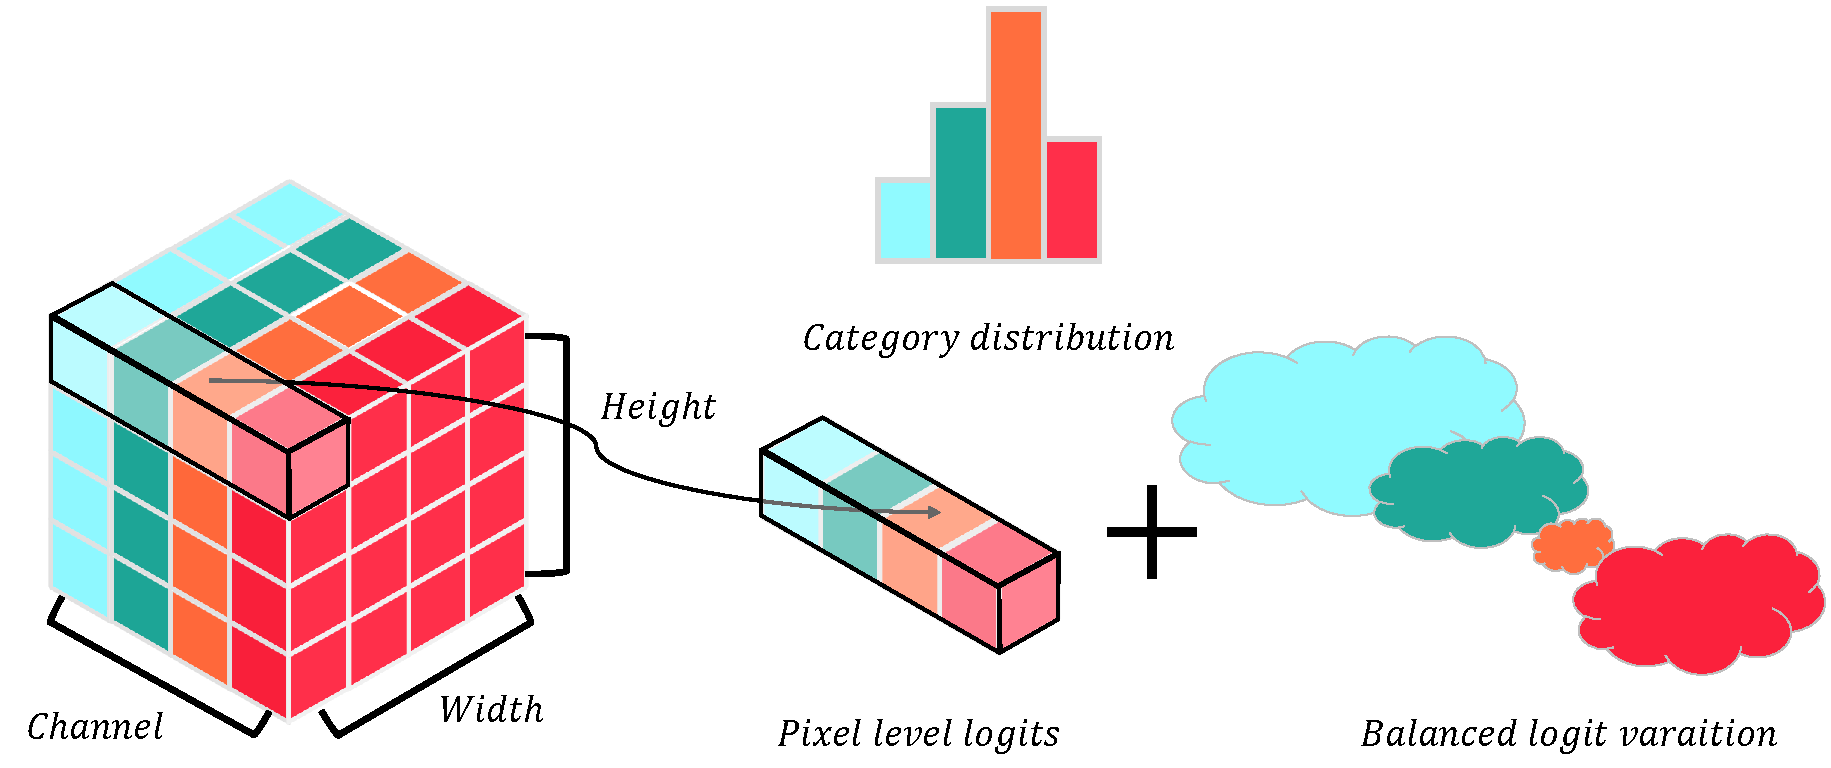
\includegraphics[width=1.0\linewidth]{figures/Methodfigure.pdf}
    \vspace{-15pt}
    \caption{%
        Diagram of the introduction of balanced logit variation, where we perturb the per-pixel logit with a category-specific noise.
        %
        The noise variance is in inverse proportion to the category scale.
    }
    \label{fig:method}
    \vspace{-10pt}
\end{figure}
%

%
Every $z_{k}^{i}$ is defined as the \textbf{logit} for the instance (\textit{i.e.}, pixel) $i$.
%
The step-by-step derivation from \cref{eq:softmax} to \cref{eq:cross_entropy} depicts a direct relationship between the $L_{CE}$ optimization and logit term $z$.
%
Logit term $z$ is critical to the long-tail problem.
%
Because the dimensionality of logit $z$ is consistent with the total number of categories and directly affects the computation of the loss, making it the most intuitive way to affect the size of the categorical area feature space.
%
Then the crux lies in how to use logit to alleviate the long-tail problem.
%
One intuitive way is simply to rescale the logit according to the category frequency~\cite{menon2021long}.
%
However, semantic segmentation is an extremely instances-intensive task, so simply rescaling the logit fixedly according to the category frequency leads to overfitting problems.


To this end, we propose to add variation into the network predictions (\textit{i.e.} $z$ here) in \cref{eq:balancing}.
\begin{equation}\label{eq:balancing}
    \hat{z}^{i}_{k} = z^{i}_{k} + \frac{c_{k}}{\max_{i=0}^{C-1}c_{i}}|\delta(\sigma)|, \quad c_{k} =\log \frac{\sum_{j=0}^{C-1}q_{j}}{q_{k}}
\end{equation}
where $q_{k}$ is the number of the instances with category $k$ and $\delta$ is a gaussian distribution with a mean of \textbf{$0$} and standard deviation of $\sigma$.
%
\cref{eq:balancing} is quite easy to understand, as it assigns smaller variation to the head categories and larger variation to the tail categories.
%
By adding this variation, which is inversely proportional to the category scale, our method can be equivalent to \textit{expanding the distribution of each instance over the feature space from a single point into a small region}.
%
Therefore, when training under this setting, we can obtain a more category-balanced feature representation space.
%
We give a more straightforward explanation of our approach in \cref{fig:method}.
%
Besides, the only hyper-parameter of \cref{eq:balancing} is the $\sigma$, making it easy to generalize to other tasks.
%
The form of variation can actually be not limited to Gaussian distribution, in the ablation experiment \cref{sec:ablation} we found that variation sampled from other distributions can also work.
%
It is noteworthy that the introduced variation is discarded at the inference stage to facilitate a confident prediction.
%
Next, we will elaborate on how to specifically apply \cref{eq:balancing} for different settings of long-tail semantic segmentation tasks.

\subsection{\method for Fully Supervised Segmentation}\label{sec:method_2}
Since the labels of the training data are available in the fully supervised semantic segmentation task, the category-by-category distribution can be obtained easily when preprocessing the data.
%
It should be noted that since the instances of the segmentation task are pixels, the number of pixels of each class needs to be counted before obtaining their distribution.
%
We present all experimental results for this task in \cref{sec:fully_super}.
%
\subsection{\method for Semi-Supervised Segmentation}\label{sec:method_3}
Semi-supervised semantic segmentation is a more challenging task, due to the fact that only a small portion of the training images are carefully labeled~\cite{zhang2020survey}.
%
A simple approach is to equate the pixel-level category distribution of the labeled images with the category distribution of the whole training set (including both the labeled and the unlabeled images).
%
This estimated distribution is quite inaccurate when the labeled/unlabeled division is very extremely unbalanced, for example, the $1/16 (186)$ partition protocols in \cref{sec:semi_exp}. 

%
Therefore, we propose an epoch-based update strategy of the distribution to make it closer to the true distribution.
%
Suppose after $n$ epochs of training, we have a model $f_{n}$. 
%
For all the unlabeled training images set $X^{u}_{image}$, we infer the labels of all the images in $X^{u}_{image}$ thus get its corresponding pseudo-label: $\hat{Y}^{u}_{image}$.
%
Thus, we calculate the number of pixels in each category by the following formula \cref{eq:cal_distribution}.
\begin{equation}\label{eq:cal_distribution}
    q_{k} = \frac{\sum_{n=1}^{N}\sum_{m=1}^{H\times W}\mathbbm{1}\left[\hat{y}_{nm}^u = k\right]}{\sum_{i=0}^{C-1}\sum_{n=1}^{N}\sum_{m=1}^{H\times W}\mathbbm{1}\left[\hat{y}_{nm}^u = i\right]}
\end{equation}
where $q_{k}$ denotes the $k$-th category frequency, $\hat{y}_{nm}^u$ denotes the $m$-th element of the $n$-th pseudo-label and $N$ is the number of the unlabeled images.

%
\cref{eq:cal_distribution} will be used to calculate the updated category distribution $\left\{q_{0}, q_{1},\cdots,q_{n-1}\right\}$ after every epoch.
%
Then we can bring this estimated distribution into \cref{eq:balancing}.
%
With this design, our approach can efficiently and consistently improve the performance of semi-supervised semantic segmentation tasks.

\subsection{\method for UDA Segmentation}\label{sec:method_4}
Unsupervised domain adaptive semantic segmentation attempts to train a model that works well on the target domain by using labeled source domain data and unlabeled target domain data.
%
Since the goal is to improve the performance of the model on the target domain, yet the images on this domain are unlabeled, this poses a tricky problem.
%

%
A widely recognized perspective is to view UDA semantic segmentation as semi-supervised semantic segmentation~\cite{zhang2021prototypical}.
%
Because the source domain data is naturally labeled, this perspective makes certain sense without considering the inter-domain gap.
%
Therefore, we can estimate the distribution of the target domain data with \cref{eq:cal_distribution}.
%

%
However, for the UDA semantic segmentation, we propose a more concise way: viewing the category distribution of the source domain data as if it were the category distribution of the target domain.
%
The data from the source domain are typical computer-rendered synthetic labeled images while the data from the target domain are generally a real-world collection of images.
%
This difference makes the images of the two domains significantly different only in terms of style, and essentially identical in terms of contextual relationships and category distribution.
%
In \cref{exp:uda} we have experimentally demonstrated that this simple estimation method works.

